% Tableaux de résultats, graphiques
% Préciser l'erreur
% Incertitudes
Ci-suit les mesures effectuées ainsi que les opérations d'analyse sur les résultats. Notons que dans le cadre de la première expérience sur le filtre "passe-bas", toute les mesures sont très correctes et soumises à une relativement faible erreur, alors que dans celle sur les filtres "passe-haut", près de la moitié des résultats ne font pas sens. Tout cela sera néanmoins discuté dans la section suivante. 

\subsection{Expérience 1 : filtre "passe-bas"}

Pour les deux volées de mesure sur ce filtre, le traitement se fait de manière similaire. Nous n'allons donc précisé que les opérations sur la première série et ne feront que mentionner les différences pour la seconde. Finalement, lors de la mise en œuvre de l'expérience, il y a eu une incompréhension menant à l'absence de la mesure de la tension d'entrée, ce qui mène à la comparaison à un modèle théorique seulement via une courbe de tendance dont nous préciserons les paramètres.

\subsubsection{Résistance de \texorpdfstring{$ 5 \ [ \Omega ] $}{TEXT}}

Dans la table suivante sont résumées nos mesures sur le circuit avec une résistance de $R = 5 \ [\Omega]$. Pour cela, on a calibré le générateur de fonction autour des fréquences désirées, ce qui est reporté dans la mesure $f$. Ensuite sont relevés par l'oscilloscope la mesure de la tension à la résistance $U$ et le décalage temporel entre la courbe d'entrée et celle sur la résistance $\Delta t$.\\
Pour le calcul du déphasage, nous utilisons la relations $\Delta t = \frac{\phi_2 - \phi_1}{\omega} \Leftrightarrow \phi_2 - \phi_1 = \phi = \Delta t \cdot \omega$, où l'on ne cherche que la valeur du déphasage $\phi$ et sachant que la pulsation $\omega = 2 \pi f$. Finalement on calcule l'inductance $L$ par $\tan \phi = \frac{\omega L}{R} \Leftrightarrow L = \frac{R}{\omega} \tan \phi$.

\begin{table}[H]
\centering
\begin{tabular}{rrrrr}
\toprule
 $f \ [Hz]$ &  $U \ [V]$ &  $\Delta t \ [ms]$ &  $\phi \ [rad]$ &  $L \ [mH]$ \\
\midrule
     10.03 &        5.600 &       0.000 &  0.000 &            0.000 \\
     20.82 &        5.640 &       0.400 &  0.052 &            2.002 \\
     50.43 &        5.560 &       0.300 &  0.095 &            1.505 \\
    110.30 &        5.400 &       0.360 &  0.249 &            1.838 \\
    213.30 &        4.960 &       0.400 &  0.536 &            2.217 \\
    509.20 &        3.480 &       0.280 &  0.896 &            1.953 \\
   1072.00 &        2.000 &       0.190 &  1.280 &            2.478 \\
   2160.00 &        1.040 &       0.110 &  1.493 &            4.719 \\
   5035.00 &        0.464 &       0.046 &  1.455 &            1.362 \\
  10150.00 &        0.226 &       0.024 &  1.531 &            1.949 \\
\bottomrule
\end{tabular}
\caption{Mesures et calculs pour le filtre "passe-bas", $R = 5 \ [ \Omega ]$}
\label{tab:p-b-5}
\end{table}

En excluant la mesure autour de $10 \ [Hz]$ car l'intervalle de temps était trop court pour être exploitable dans le calcul de l'inductance, nous obtenons une moyenne à $L \approx 2.225 \ [mH]$ avec un écart-type de $\sim 0.937 \ [mH]$. À noter que $L = 3 \ [mH]$ du fabricant est compris dans l'écart-type, néanmoins il y a quand même un grand écart avec la moyenne.\\ \\
Pour visualiser ces données, nous avons fait un premier graphe de l'intensité selon la fréquence. Comme la plage de donnée est grande, cela se fait sur une échelle logarithmique sur les deux axes. Les points de mesure sont obtenus par la tensions aux bornes de la résistance et la loi d'Ohm $U = RI \Leftrightarrow I = \frac{U}{R}$. Pour le modèle, il y a la relation pour un circuit $RL$ que $I = \frac{U_{in}}{\sqrt{R^2 + (\omega L)^2}}$. On utilise alors une méthode des moindres carrés non-linéaire afin de trouver une valeur de $U_{in}$ qui correspond donc à la tension d'entrée qui aurait dû être mesurée. Celle-ci fut  donc calculée à $U_{in} \approx 5.696 \ [V]$ en ayant fixé l'inductance du circuit à la moyenne calculée plus haut.\\
Afin de calculer la fréquence de coupure du filtre "passe-bas", il a fallu construire les asymptotes du graphe sur cette échelle logarithmique, puis nous avons calculé leurs intersections en itérant sur les points calculés et voir quand leur écart était moindre ce qui nous donne une fréquence de coupure $f_c \approx 443.248 \ [Hz]$. Pour ce graphe-là, on a pu le faire via nos points de mesure.\\

\begin{invsummary}
Pour calculer les asymptotes, il a fallu jongler entre les équations de droite et les exponentielle. Pour celle horizontale tout d'abord, il a suffit de tracer une droite à la hauteur du premier point.\\
Pour celle oblique, on a commencé par calculer la pente $m$ entre les points désirés avec le premier $P_1(f_1;I_1)$ et le second $P_2(f_2;I_2)$ (donc $f_1 < f_2$). Comme c'est en échelle logarithmique on prend le logarithme (note : dans ce qui suit $\log$ désigne celui en base 10 utilisé dans l'analyse informatique des données) de chaque valeur et on calcule la pente de manière standard $m = \frac{\log (I_2) - \log (I_1)}{\log (f_2) - \log (f_1)}$. L'ordonnée à l'origine $h$ se calcule selon la même logique en prenant un des points $h = \log (I_1) - m \cdot \log (f_1)$. La droite sera alors sur un intervalle $[a;b]$ les points $(10^{[a;b]};10^{m \cdot [a;b] + h})$. On a pris comme points les deux derniers du graphe afin d'avoir la bonne asymptote.\\
À noter que pour le filtre "passe-haut", l'asymptote horizontale se fait par le dernier point et celle oblique par les premiers points.
\end{invsummary}
Pour le déphasage, seul la fréquence est sur une échelle logarithmique. Nous avons mis le déphasage obtenu par les calculs sur la mesure et celui calculé par le modèle $\tan \phi = \frac{\omega L}{R} \Leftrightarrow \phi = \arctan \left( \frac{\omega L}{R} \right)$. La valeur de $L$ fixée est toujours la même.

\begin{minipage}{.5\textwidth}
\begin{figure}[H]
\centering
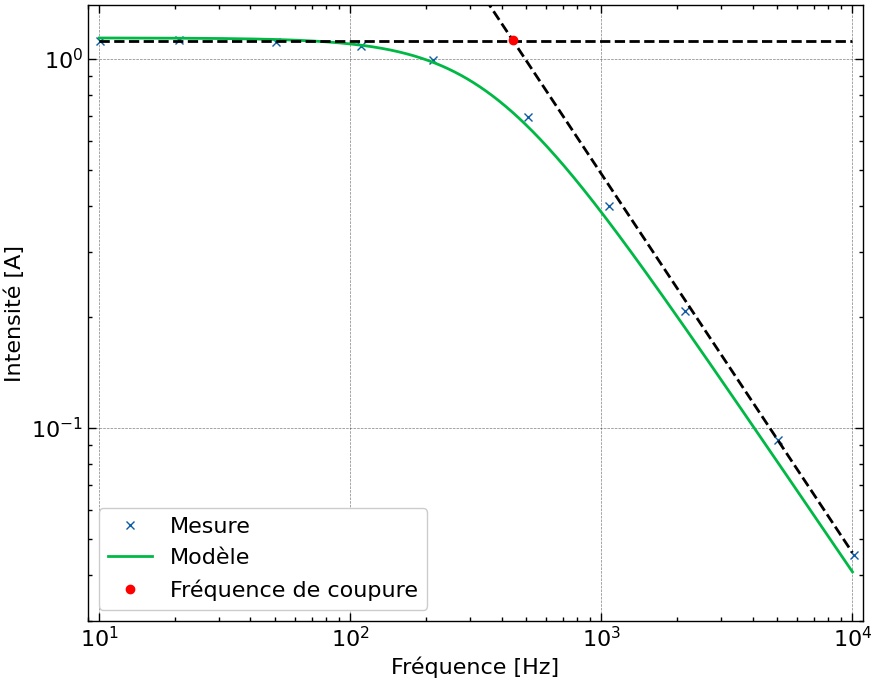
\includegraphics[scale=0.35]{i_pb_5.png}
\caption{Intensité, "passe-bas", $R = 5 \ [ \Omega ]$}
\end{figure}
\end{minipage}
\begin{minipage}{.5\textwidth}
\begin{figure}[H]
\centering
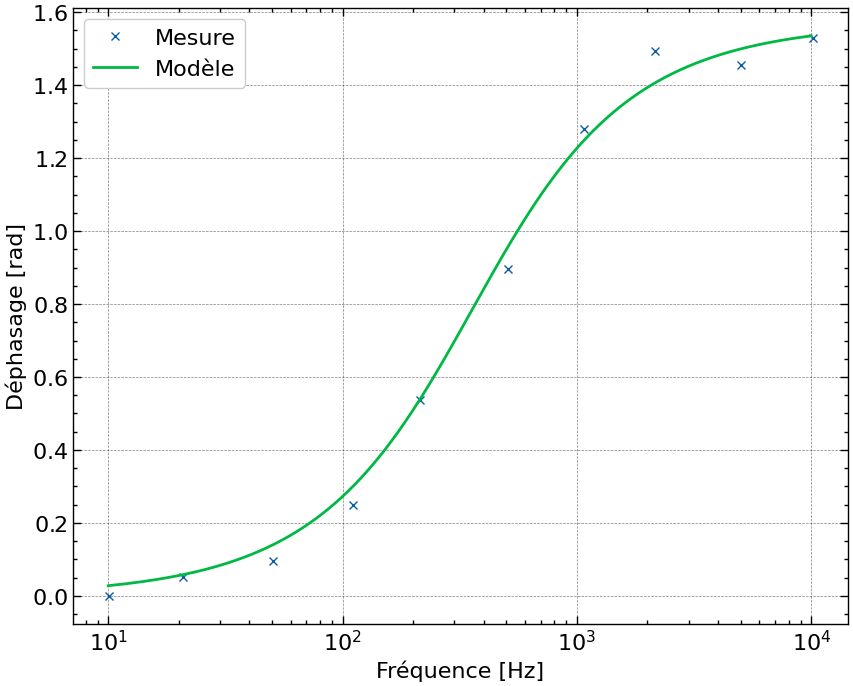
\includegraphics[scale=0.35]{p_pb_5.png}
\caption{Déphasage, "passe-bas", $R = 5 \ [ \Omega ]$}
\end{figure}
\end{minipage}

\subsubsection{Résistance de \texorpdfstring{$ 50 \ [ \Omega ] $}{TEXT}}

Pour le tableau suivant, la résistance $R=50 \ [\Omega]$. Les méthodes de calcul sont les même. L'inductance moyenne est cette fois-ci calculée en excluant les deux premières mesures qui sont manifestement inexploitables. On obtient via ces considérations une inductance $L \approx 3.463 \ [mH]$ avec un écart-type de $\sim 0.764 \ [mH]$. On est donc un peu plus proche de la valeur du fabricant, mais cela reste assez éloigné, et de plus cela est aux antipodes des mesures avec $R=5 \ [\Omega]$.

\begin{table}[H]
\centering
\begin{tabular}{rrrrr}
\toprule
 $f \ [Hz]$ &  $U \ [V]$ &  $\Delta t \ [ms]$ &  $\phi \ [rad]$ &  $L \ [mH]$ \\
\midrule
     10.32 &         8.32 &       0.000 &  0.000 &            0.000 \\
     21.03 &         8.32 &       0.400 &  0.053 &           20.019 \\
     49.58 &         8.32 &       0.100 &  0.031 &            5.002 \\
    119.00 &         8.32 &       0.080 &  0.060 &            4.005 \\
    217.80 &         8.16 &       0.080 &  0.109 &            4.016 \\
    505.30 &         8.00 &       0.050 &  0.159 &            2.521 \\
   1187.00 &         7.68 &       0.056 &  0.418 &            2.975 \\
   2170.00 &         6.52 &       0.048 &  0.654 &            2.814 \\
   5045.00 &         4.00 &       0.035 &  1.109 &            3.173 \\
  10680.00 &         2.06 &       0.020 &  1.342 &            3.201 \\
\bottomrule
\end{tabular}
\caption{Mesures et calculs pour le filtre "passe-bas", $R = 50 \ [ \Omega ]$}
\label{tab:p-b-50}
\end{table}

Quant aux graphes, mentionnons juste que sur ceux-ci, l'inductance fixée est celle du fabricant de $L=3 \ [mH]$. Cela à mené au calcul d'une tension d'entrée $U_{in} \approx 8.310 \ [V]$ et la fréquence de coupure $f_c \approx 2204.669 \ [Hz]$.

\begin{minipage}{.5\textwidth}
\begin{figure}[H]
\centering
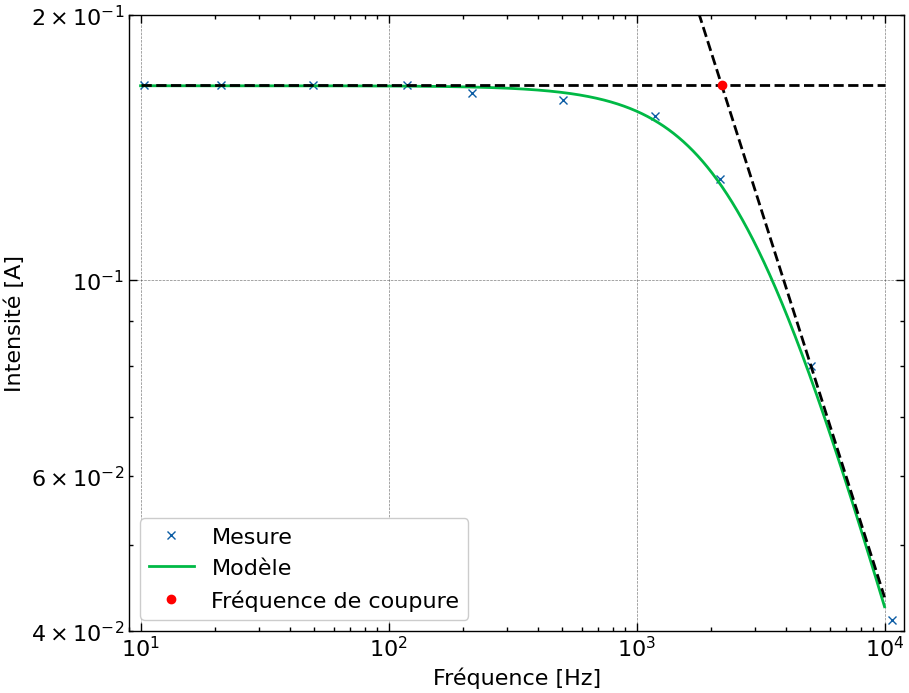
\includegraphics[scale=0.35]{i_pb_50.png}
\caption{Intensité, "passe-bas", $R = 50 \ [ \Omega ]$}
\end{figure}
\end{minipage}
\begin{minipage}{.5\textwidth}
\begin{figure}[H]
\centering
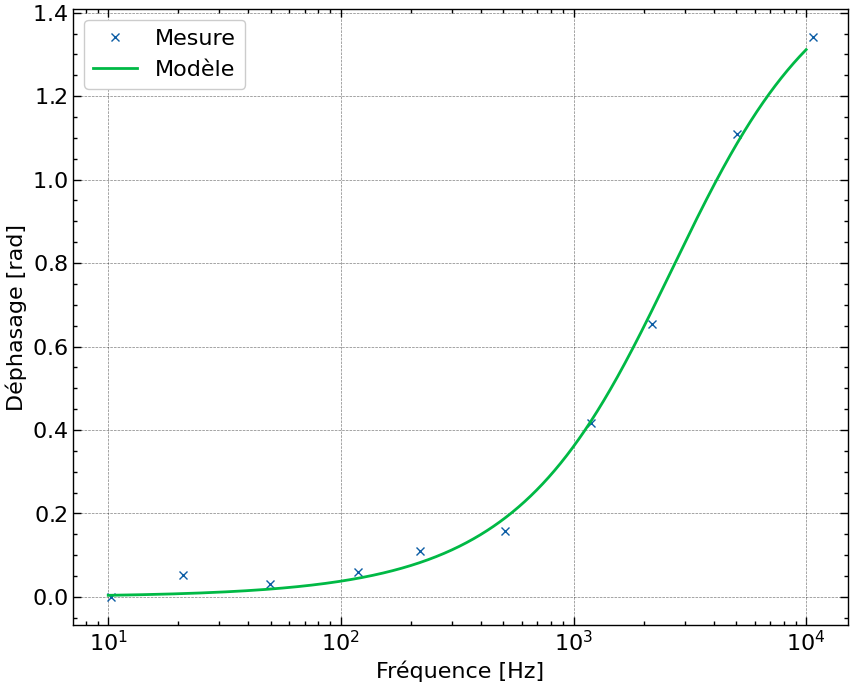
\includegraphics[scale=0.35]{p_pb_50.png}
\caption{Déphasage, "passe-bas", $R = 50 \ [ \Omega ]$}
\end{figure}
\end{minipage}

\subsection{Expérience 2 : filtre "passe-haut"}

Pour ces mesures sur le filtre "passe-haut", nous ne prîmes qu'une volée sur un résistance $R= 50 \ [\Omega]$. Notons que tout le matériel à été changé car ce sont deux jours de mesures différents. Cette fois, la tension d'entrée a bien été mesurée, néanmoins, dû a un problème matériel, la mesure sur l'oscilloscope était presque impossible quand les fréquences étaient trop basses ce qui donne près de la moitié des mesures inexploitables.

\subsubsection{Résistance de \texorpdfstring{$ 50 \ [ \Omega ] $}{TEXT}}

Les mesures sont globalement les mêmes que sur le filtre "passe-bas". Notons néanmoins que dû au comportement étrange de l'oscilloscope et au paradigme apparaissant aux premières mesures, le décalage temporel $\Delta t$ à été mesuré dans sa valeur la plus grande, et donc pour avoir la phase la plus petite il a fallu rectifier le calcul par $2\pi$, en résumé $\phi := \phi - 2\pi$. Pour le calcul de la capacité, on utilise la relation $\tan \phi = - \frac{1}{\omega R C} \Leftrightarrow C = - \frac{1}{\omega R \tan \phi}$.

\begin{table}[H]
\centering
\begin{tabular}{rrrrrr}
\toprule
 $f \ [Hz]$ &  $U \ [V]$ & $U_{in} \ [V]$ &  $\Delta t \ [ms]$ &  $\phi \ [rad]$ &  $C \ [\mu F]$ \\
\midrule
     5.102 &        0.222 &           10.20 &    100.0000 & -3.078 &      -9721.527 \\
    10.950 &        0.280 &           10.10 &     52.4000 & -2.678 &       -581.496 \\
    21.100 &        0.184 &           10.20 &     29.0000 & -2.439 &       -177.986 \\
    51.870 &        0.344 &           10.00 &     13.6000 & -1.851 &        -17.648 \\
   104.300 &        0.620 &            9.92 &      6.2400 & -2.194 &        -21.930 \\
   208.000 &        0.848 &            9.92 &      3.2800 & -1.997 &         -6.940 \\
   516.000 &        1.860 &            9.92 &      1.4400 & -1.615 &         -0.270 \\
  1034.000 &        3.300 &            9.92 &      0.7600 & -1.346 &          0.705 \\
  2185.000 &        5.880 &           10.10 &      0.3800 & -1.066 &          0.804 \\
  5060.000 &        8.400 &            9.92 &      0.1800 & -0.560 &          1.002 \\
 10980.000 &        9.200 &            9.76 &      0.0880 & -0.212 &          1.346 \\
 20460.000 &        9.200 &            9.36 &      0.0476 & -0.164 &          0.940 \\
\bottomrule
\end{tabular}
\caption{Mesures et calculs pour le filtre "passe-haut", $R = 50 \ [ \Omega ]$}
\label{tab:p-h-50}
\end{table}

En excluant les valeurs incohérentes ($C<0$), nous obtenons une moyenne à $C \approx 0.960 \ [\mu F]$ avec un écart-type de $\sim 0.219 \ [\mu F]$, ce qui est raisonnable vis à vis des spécifications du fabricant disant $1 \ [\mu F]$, mais moins bon quand on considère la mesure au multimètre annonçant $1.15 \ [\mu F]$.\\ \\
Pour l'intensité, la démarche est toujours la même, quoique pour le modèle nous utilisons cette fois les mesures de $U_{in}$ et la formule $I = \frac{U_{in}}{\sqrt{R^2 + \left(\frac{1}{\omega C}\right)^2}}$. Nous y avons aussi fait passer une courbe de tendance par les valeurs calculées par $U_{in}$ en fixant $U_{in} \approx 9.725 \ [V]$. Notons également que les asymptotes pour le calcul de la fréquence de coupure s'appuie également sur ces valeurs et donne $f_c \approx 2700.421 \ [Hz]$. Pour le déphasage, le modèle se base sur $\tan \phi = - \frac{1}{\omega R C} \Leftrightarrow \phi = \arctan \left( -\frac{1}{\omega R C} \right)$.

\begin{minipage}{.5\textwidth}
\begin{figure}[H]
\centering
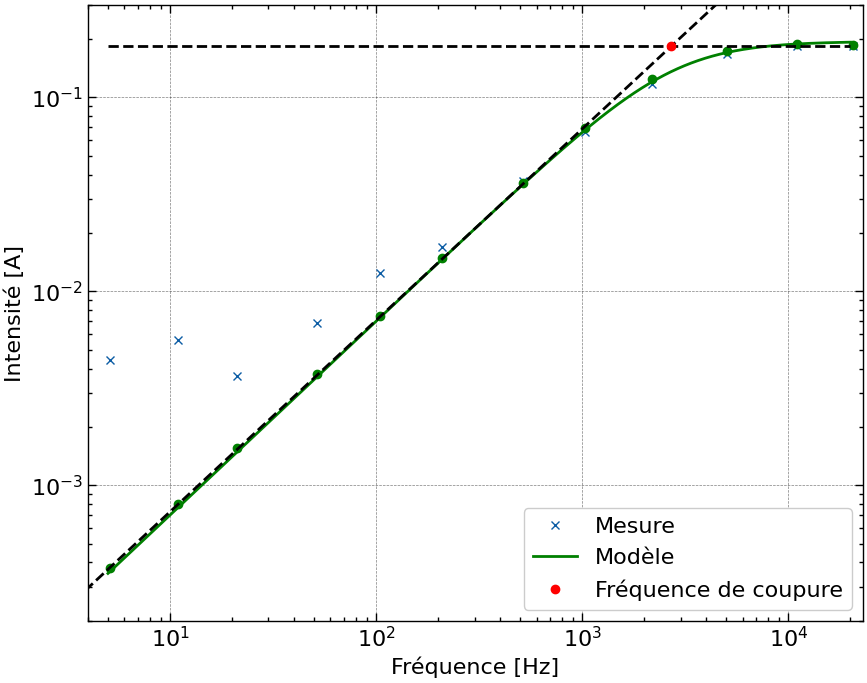
\includegraphics[scale=0.35]{i_ph_50.png}
\caption{Intensité, "passe-haut", $R = 50 \ [ \Omega ]$}
\end{figure}
\end{minipage}
\begin{minipage}{.5\textwidth}
\begin{figure}[H]
\centering
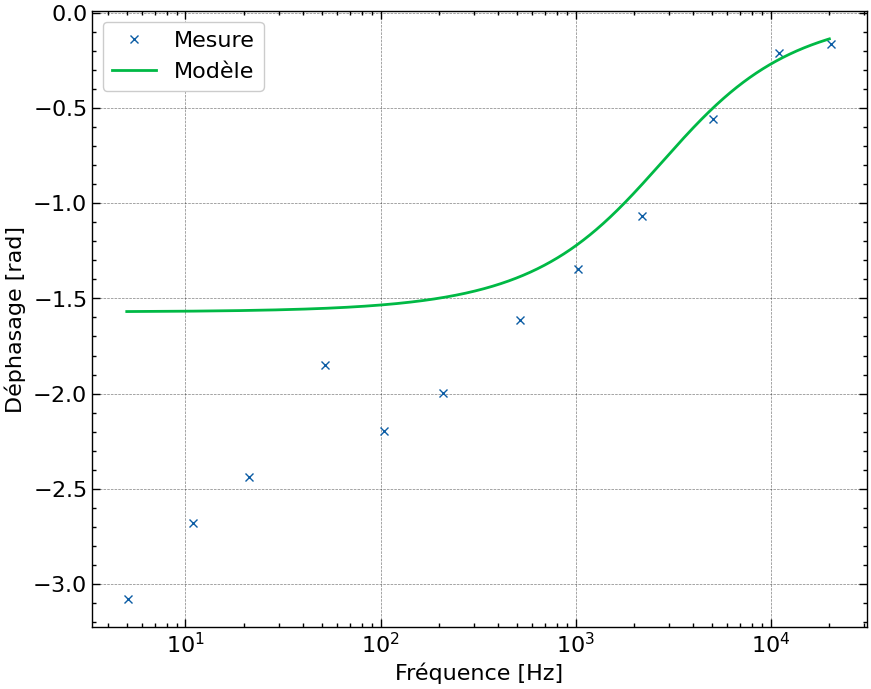
\includegraphics[scale=0.35]{p_ph_50.png}
\caption{Déphasage, "passe-haut", $R = 50 \ [ \Omega ]$}
\end{figure}
\end{minipage}